% Generated from tex/chapters/ch04/08_構築技術.tex for the SWEBOK structure tree
\subsubsection{テストファーストプログラミング}

テストファーストプログラミングは、コードを書く前にテストケースを書く開発スタイルである。現在のコードベースでそのテストは失敗する。その後、テストが通るようにコードを書く。テストが通ったら、必要に応じてリファクタリングし、設計を整える。

この方法は、テスト駆動開発としても知られる。テストを先に書くことで、プログラマは要求と設計を先に考える。これにより、要求や設計の問題が早く表面化する。欠陥も早く発見され、修正しやすい。

\begin{figure}[htbp]
\centering
\IfFileExists{assets/generated_figures/ch04/fig-ch04-14.png}{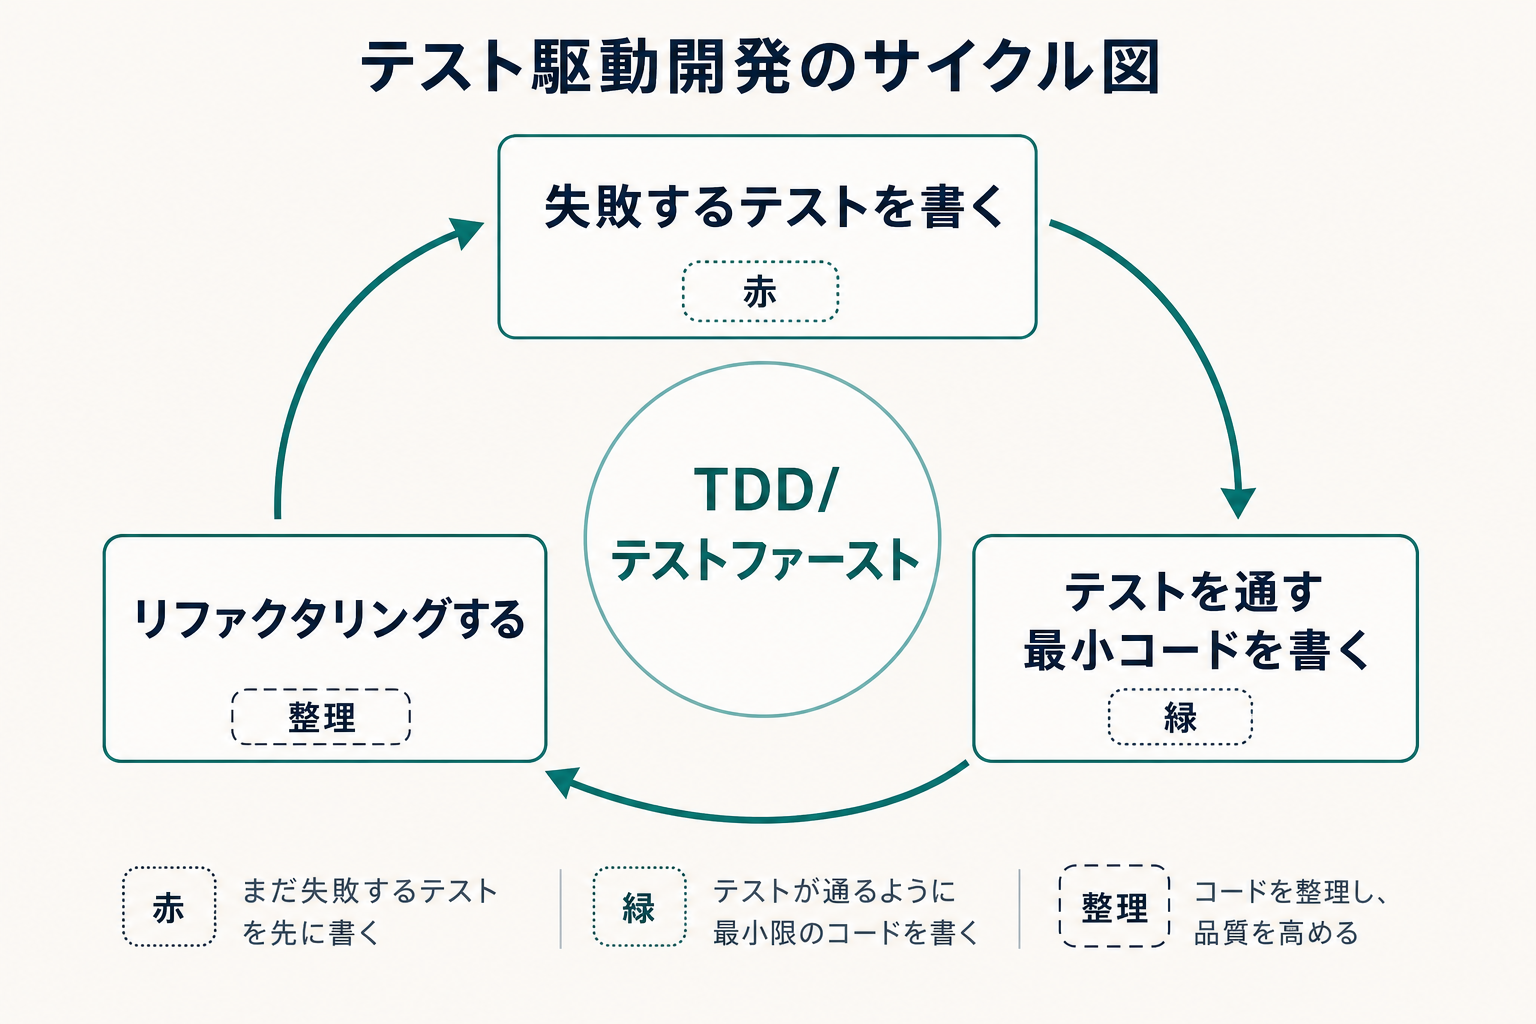
\includegraphics[width=0.96\linewidth]{assets/generated_figures/ch04/fig-ch04-14.png}}{\fbox{\parbox[c][48mm][c]{0.9\linewidth}{\centering 画像生成待ち\\テスト駆動開発のサイクル図}}}
\caption{テスト駆動開発のサイクル図}
\label{fig:ch04-14}
\end{figure}
